%%%%%%%%%%%%%%%%%%%%% Chapter 6 %%%%%%%%%%%%%%%%%%%%%%%%%%%%%%%%%
% Privacy Attacks: Breaking the System
%%%%%%%%%%%%%%%%%%%%%%%%%%%%%%%%%%%%%%%%%%%%%%%%%%%%%%%%%%%%%%%%%
\motto{To build a truly robust defense, the Trustworthy AI Architect must first learn to think like the adversary.}

\chapter{Privacy Attacks: Breaking the System}
\label{chap:privacy_attacks}

\abstract{In this chapter, we step into the adversary's shoes to understand the most common privacy and security attacks against AI systems. While previous chapters provided the mathematical shields, here we explore the weapons: Membership Inference (MIA), Model Inversion, and Data Poisoning. We categorize attacks by their goals and phases, and reference early research on poisoning rates to show how even minor data corruptions can undermine system integrity. Understanding these vulnerabilities is critical for establishing a realistic threat model for any AI deployment.}

\section{The Adversary Is Real}
\label{sec:adversary_is_real}

Imagine deploying a fraud detection model for a major bank. You've used Federated Learning to keep data decentralized and Differential Privacy to add mathematical guarantees. Yet, without a realistic threat model, the system remains vulnerable to sophisticated attackers who aim to steal customer identities or corrupt model behavior.

AI systems face unique threats compared to traditional software because the data is "memorized" within the model's weights. We categorize these threats into two main categories:

\begin{description}
  \item[Privacy Attacks:] 
        The goal is to steal information about the training data or the model itself (e.g., Membership Inference, Model Inversion).
  \item[Security Attacks:]
        The goal is to break the functionality or reliability of the model (e.g., Data Poisoning, Evasion).
\end{description}

\section{The Attack Landscape}
\label{sec:attack_landscape}

Table~\ref{tab:attack_taxonomy} outlines the primary attack vectors in modern machine learning.

\begin{table}
\caption{Taxonomy of AI Privacy and Security Attacks}
\label{tab:attack_taxonomy}
\begin{tabular}{p{3.5cm}p{5cm}p{2cm}}
\hline\noalign{\smallskip}
Attack Type & Goal & Phase \\
\noalign{\smallskip}\svhline\noalign{\smallskip}
Membership Inference & Determine if a specific record was in the training set. & Inference \\
Model Inversion & Reconstruct sensitive input data from outputs. & Inference \\
Data Poisoning & Inject malicious data to corrupt the model. & Training \\
Model Extraction & Steal model functionality by querying it. & Inference \\
\noalign{\smallskip}\hline\noalign{\smallskip}
\end{tabular}
\end{table}

\section{Membership Inference Attack (MIA)}
\label{sec:mia}

The goal of a Membership Inference Attack is to answer the question: \textit{``Was Patient X's record used to train this model?''} If the answer is yes, then X is revealed to belong to a specific cohort (e.g., a dataset of cancer patients), which constitutes a major privacy breach as demonstrated by Shokri et al. \cite{shokri2017}.

\paragraph{How It Works:} Machine learning models often exhibit higher confidence levels and lower loss values on data they have seen during training compared to unseen data. An attacker can build a "shadow model" to mimic the target model's behavior, identify the confidence thresholds that distinguish members from non-members, and then query the target victim.

\begin{figure}[h]
\centering
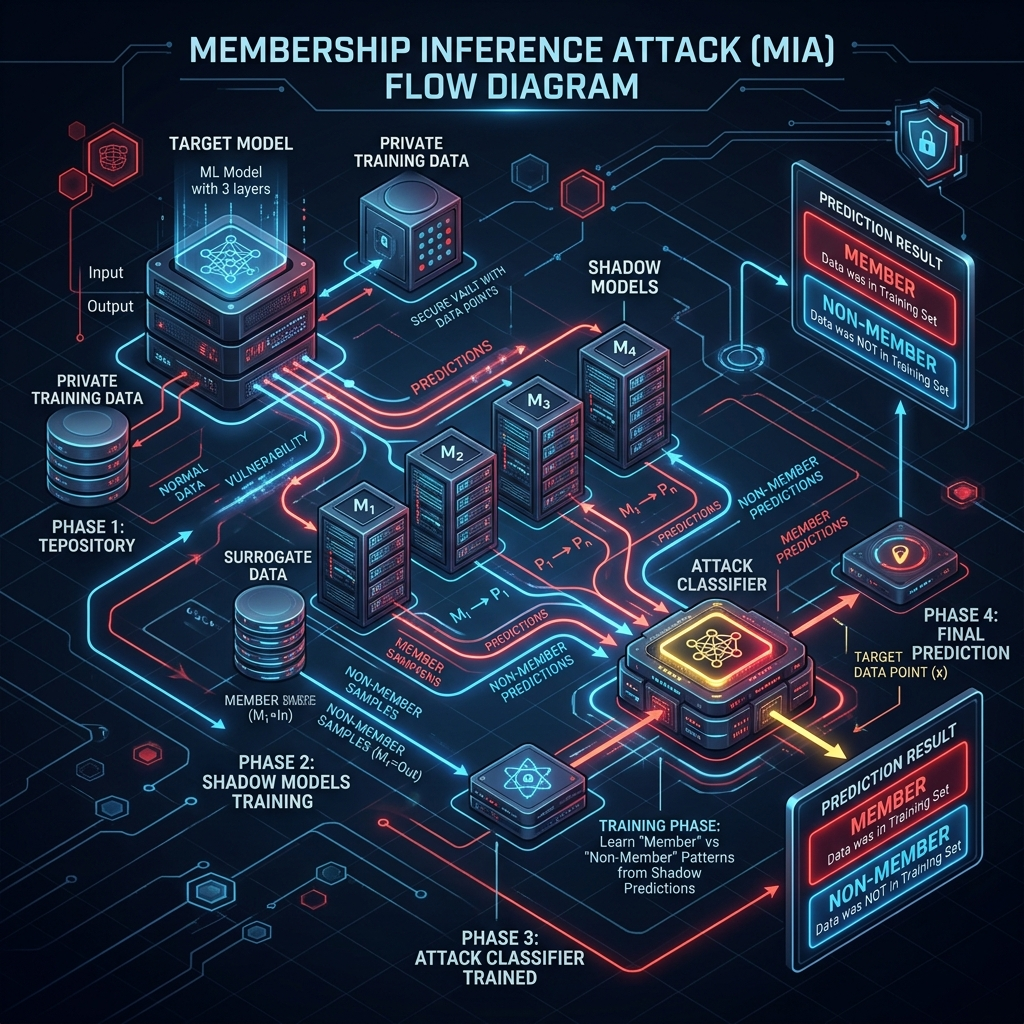
\includegraphics[width=\textwidth]{figures/ch6_mia.png}
\caption{Membership Inference Attack (MIA) Flow Diagram: Illustrating the use of shadow models and an attack classifier to identify training set members.}
\label{fig:ch6_mia}
\end{figure}

\section{Model Inversion and Gradient Leakage}
\label{sec:model_inversion}

Model Inversion aims to reconstruct sensitive input data, such as faces or genomic sequences, from the model's outputs or its gradients. In Federated Learning environments, "deep leakage" from gradients \cite{zhu2019} can reveal recognizable private images if the updates are not correctly obscured with noise (DP-SGD) or multi-party computation.

\section{Data Poisoning: Corrupting the Source}
\label{sec:data_poisoning}

Data Poisoning occurs during the training phase. An attacker injects malicious samples into the training set to influence the model's final behavior. 

\begin{svgraybox}
\textbf{Research Insight (ACOMP 2020) \cite{trantruong2020}:} Early research by Tran-Truong et al. on poisoning attacks found that even a poisoning rate of less than 5 percent can significantly degrade model accuracy or introduce specific "backdoors." For example, a poisoned fraud model could be trained to ignore all transactions from a specific attacker's account while appearing perfectly normal for all other queries.
\end{svgraybox}

\section{Conclusion}
\label{sec:conclusion_attacks}

Part II has provided the essential "Data Defense" toolkit. We have seen how simple anonymization fails (Chapter 4), how Differential Privacy provides a mathematical shield (Chapter 5), and the specific attacks that this shield must withstand (Chapter 6). 

In Part III, we will expand our perspective from single-point data defense to \textbf{Secure Distributed Systems}, exploring how to orchestrate training across multiple locations without ever moving the raw data through \textbf{Federated Learning}.


